\documentclass[11pt]{article}

%%%%%%%%%%%%%%Include Packages%%%%%%%%%%%%%%%%%%%%%%%%%%
\usepackage{xcolor}
\usepackage{mathtools}
\usepackage[a4paper, total={6in, 8in}, margin=1.25in]{geometry}
\usepackage{amsmath}
\usepackage{amssymb}
\usepackage{paralist}
\usepackage{rsfso}
\usepackage{amsthm}
\usepackage{wasysym}
\usepackage[inline]{enumitem}   
\usepackage{hyperref}
\usepackage{tocloft}
\usepackage{titlesec}
\usepackage{colortbl}
\usepackage{wrapfig}
\usepackage{pdfpages}
%%%%%%%%%%%%%%%%%%%%%%%%%%%%%%%%%%%%%%%%%%%%%%%%%%%%%%%%



\begin{document}

\begin{wrapfigure}[10]{r}{0.42\textwidth}
  \begin{center}
  \vspace{-15pt}
    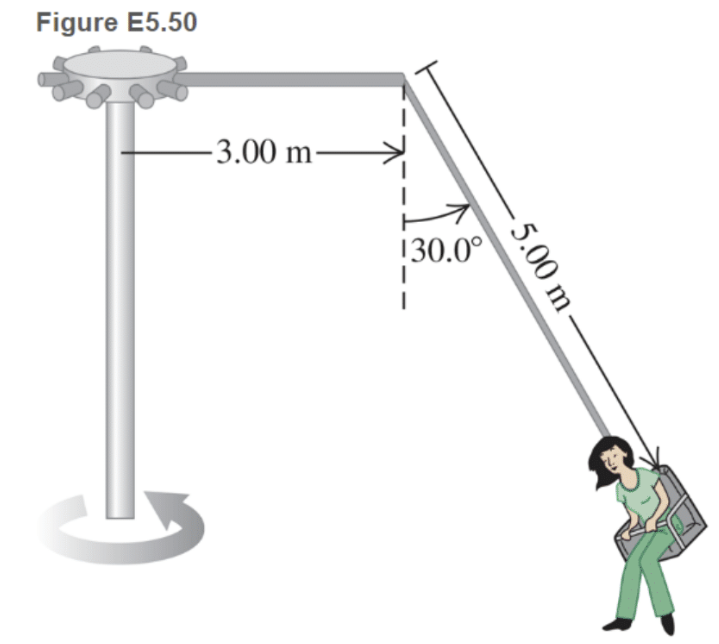
\includegraphics[scale=0.38]{swing}
  \end{center}
\end{wrapfigure}
\Large \noindent \textbf{Physics 1A Discussion (Week 3)}\\
\normalsize
Department of Physics and Astronomy, UCLA\\
\noindent\rule{8cm}{0.4pt}\\
%\begin{center}
%
\includegraphics[scale=0.55]{pull}
%\end{center}
Jinyan is trying to swing a $2\, \text{kg}$ pumpkin in a huge clockwise circular path by using a rope attached to the pumpkin. The pumpkin maintains an instantaneous linear speed $v = 5\,$m/s in its circular motion, and is subject to the gravitational force by gravity, and the tension force by the rope. The radius of the circular path is $R =1\,$m. \\
\hfill\break

\noindent \textbf{Part 1}: Draw the free-body diagram of the pumpkin when it is at the top and at the bottom of the circular path.\\


\noindent Top: \qquad\qquad\qquad\qquad\qquad\qquad\qquad
Bottom:
\hfill\break\hfill\break\hfill\break
\hfill\break\hfill\break\hfill\break

\noindent \textbf{Part 2}: At the bottom of the circular path, compute the tension force that the rope exerts on the pumpkin. 
(\textit{Hint: The total force acting on the pumpkin should help it to maintain its circular motion.)}
\hfill\break\hfill\break\hfill\break
\hfill\break\hfill\break\hfill\break
\hfill\break\hfill\break\hfill\break

\noindent \textbf{Part 3}: At the top of the circular path, find the minimal speed that the pumpkin needs to have in order to maintain its circular motion. (\textit{See hints on the back of the page.})


\newpage
\noindent\textbf{Hints for part 3}: Intuitively, if the pumpkin moves too slow at the top of the trajectory, it will just fall down and hit Jinyan instead of going in a full circle. Mathematically, we have the centripetal motion formula 
$F_{\text{NET}}  = m v^2/R\,,$ so the minimal speed occurs when $F_{\text{NET}}$ is minimal. Based on the free-body diagram that you have for the pumpkin at the top of its trajectory, there should be a way for you to change (the magnitude of) one of the forces to minimize the net force acting on the pumpkin. 
\hfill\break

\noindent\textbf{Part 4}: Based on the given information in the problem, will the pumpkin be able to maintain its circular path? Why?\\
\hfill\break\hfill\break\hfill\break
\hfill\break\hfill\break\hfill\break

\noindent\textbf{Part 5}: At the top of the circular path, compute the tension force that the rope exerts on the pumpkin. \\
\hfill\break\hfill\break\hfill\break
\hfill\break\hfill\break\hfill\break
\hfill\break\hfill\break\hfill\break

\noindent\textbf{Part 6}: Find the angular velocity and the period of the pumpkin in this circular path. 
\hfill\break\hfill\break\hfill\break
\hfill\break\hfill\break\hfill\break
\hfill\break\hfill\break\hfill\break

\noindent\textbf{Part 7}: Draw the free-body diagram of the pumpkin when it travels to the position as shown in the front-page figure. (\textit{Hint: Does the tension force by the rope point to the center of the circular path in this case?})

\newpage
\noindent Solutions:\\

\noindent\textbf{Part 1}: 
\begin{center}
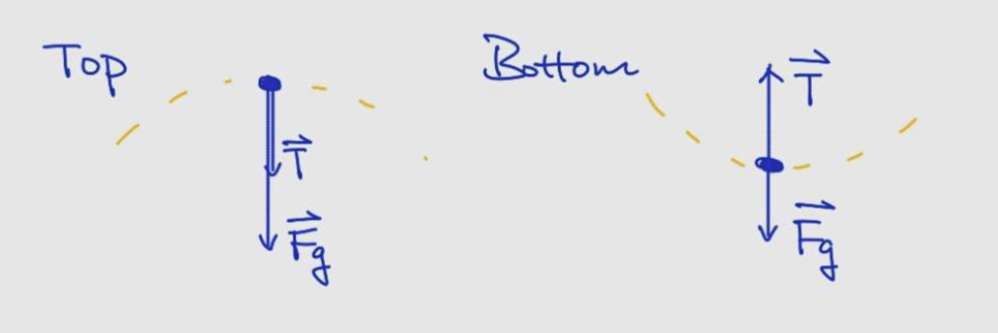
\includegraphics[scale=0.5]{fbd}
\end{center}
\noindent\textbf{Part 2}:\\
At the bottom of the circular path, we have a tension force pointing upward and a gravitational force pointing downward acting on the pumpkin, these two are the only physical forces acting on the pumpkin, nothing else. The sum of the two physical forces ($\vec{T}$ and $\vec{F}_g$) should give us a centripetal force (which is the net force acting on the pumpkin). Since the pumpkin is at the bottom, we expect the centripetal force to point upward towards the center of the circular path. Thus we can write down the $y$-component of all the forces, 
\begin{align*}
\frac{mv^2}{R} = T- mg\,.
\end{align*}
It is important to have the correct sign in this equation. Then we just need to isolate $T$ can plug in the numbers,  
\begin{align*}
T = \frac{mv^2}{R} + mg = \frac{(2\,\text{kg})\cdot (5\,\text{m/s})^2}{(1\,\text{m})} + (2\,\text{kg})\cdot(9.8\,\text{m/s}^2) = 69.6\,\text{N}\,.
\end{align*}
The tension force is $69.6$ Newtons.\\

\noindent\textbf{Part 5}:\\
Before we do parts 3 and 4, let us look at part 5, which also asks for the tension force, but at the top of the pumpkin's trajectory. At the top of the circular path, now both tension force and gravitational forces are pointing downward. The sum of the two physical forces ($\vec{T}$ and $\vec{F}_g$) should give us a centripetal force (which is the net force acting on the pumpkin). Since the pumpkin is at the top, we expect the centripetal force to point down towards the center of the circular path. Thus we can write down the $y$-component of all the forces, 
\begin{align*}
-\frac{mv^2}{R} = -T- mg\,. \tag{*}
\end{align*}
All quantities have negative sign in front, because they are all pointing down. Then we just need to isolate $T$ can plug in the numbers,  
\begin{align*}
T = \frac{mv^2}{R} - mg = \frac{(2\,\text{kg})\cdot (5\,\text{m/s})^2}{(1\,\text{m})} - (2\,\text{kg})\cdot(9.8\,\text{m/s}^2) = 30.4\,\text{N}\,.
\end{align*}
The tension force is $30.4$ Newtons.\\

\noindent\textbf{Part 3}:
The physics here is that the tension is not the same throughout the circular path of the pumpkin, this is because you do not need to put in the same amount the force to spin the pumpkin when the pumpkin is at different location in its circular path. When the pumpkin is at the bottom, you generally need to pull the rope harder to pull it up, but when the pumpkin is at the top, gravity will help you to pull it down. This idea is essential for part 3, where we want to minimize the speed of the pumpkin. \\

Intuitively, when the pumpkin is at the top of the trajectory, gravitational force is pulling it down, so we do not even need to put in extra tension to pull it down in order to maintain the circular motion, so we can simply set $T = 0\,$N. This would minimize the speed of the pumpkin, as you can imaging: If I pull the rope harder, spinning the pumpkin harder, the pumpkin should spin faster, so if the tension is low, pumpkin spins slower.\\

Mathematically, we look at equation (*) that we derived in part 5, and we multiply $-1$ to both sides of the equation and get
\begin{align*}
\frac{mv^2}{R} = T + mg\,,
\end{align*}
from which we see that, to minimize $v$, we can only change $T$ because the mass $m$ and the gravitational acceleration $g$ always stay the same, the radius of the circular path should also stay the same. Thus minimizing $T$ minimizes $v$, we set $T = 0$, and find
\begin{align*}
\frac{mv^2}{R} = mg\,,
\end{align*}
from here we plug in the numbers and find
\begin{align*}
v = \sqrt{\frac{mgR}{m}} = 3.13\,\text{m/s}\,.
\end{align*}
The minimal speed the pumpkin should have is $3.13\,$m/s. For any number below $v=3.13\,$m/s, the pumpkin will not be able to maintain its circular path, as the gravitational force is pulling it too hard that the rope will slack and the pumpkin just fall down. \\

\noindent\textbf{Part 4}:\\
As given in the problem, the pumpkin is spinning with $5\,$m/s which is faster than $3.13\,$m/s, so the pumpkin is able to maintain its circular path.\\

\noindent\textbf{Part 6}:\\
To find the angular velocity, we use the formula
\begin{align*}
\omega = \frac{v}{r} = \frac{5\,\text{m/s}}{1\,\text{m}} = 5\,\text{rad/s}\,.
\end{align*} 
The period is defined by the time it takes to go one full circle, which corresponds to the angle $\theta = 2\pi$, or the distance traveled $d = 2\pi R$ being the circumference of the circle. We can find the period $T$ using either way, starting with the easy one, time is distance over velocity,
\begin{align*}
T = \frac{2\pi R}{v} = 1.26\,\text{s}\,.
\end{align*}
Or using the angle, again, time is angle over angular velocity, 
\begin{align*}
T = \frac{2\pi}{\omega} = 1.26\,\text{s}\,.
\end{align*}


\noindent\textbf{Part 7}:\\
The key point for this question is that my hand (holding the rope) is not the center of the circular path. The tension force points in the direction of the rope, and thus points towards my hand, but that is not the center of the circular path. Instead, if we add gravitational force to the tension, and get the net force (centripetal force), the net force points towards the center of the circular path. This is the key feature of a centripetal force for circular motion. \\

Physically, this makes sense because when one is spinning a heavy object, his hand needs to be moving in a smaller circle (sort of), and thus cannot be the center of the circular path. If he puts his hand stationary in space, there is no way he can spin a heavy object in a perfect circular path.

\begin{center}
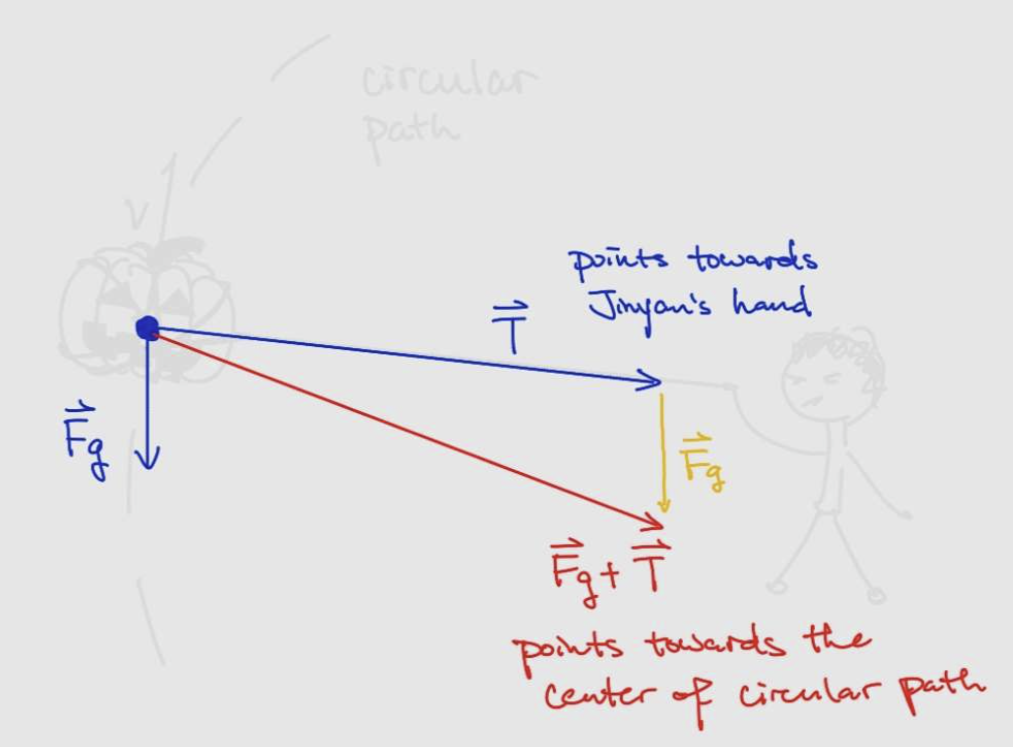
\includegraphics[scale=0.39]{spin}
\end{center} 
 
\end{document}


